% !TEX root = ./main.tex
\documentclass[a4paper]{article}
% Course language: use [english] or [german].
\usepackage[german]{ajnotes}
\title{\textbf{Mikrooekonomik — Woche 3 Angebot und Nachfrage}}
\begin{document}
    \maketitle
    % Attach the given problem sheet: drop it in this folder as sheet.pdf and
    % un-comment the next line (pdfpages is already loaded by the preamble).
    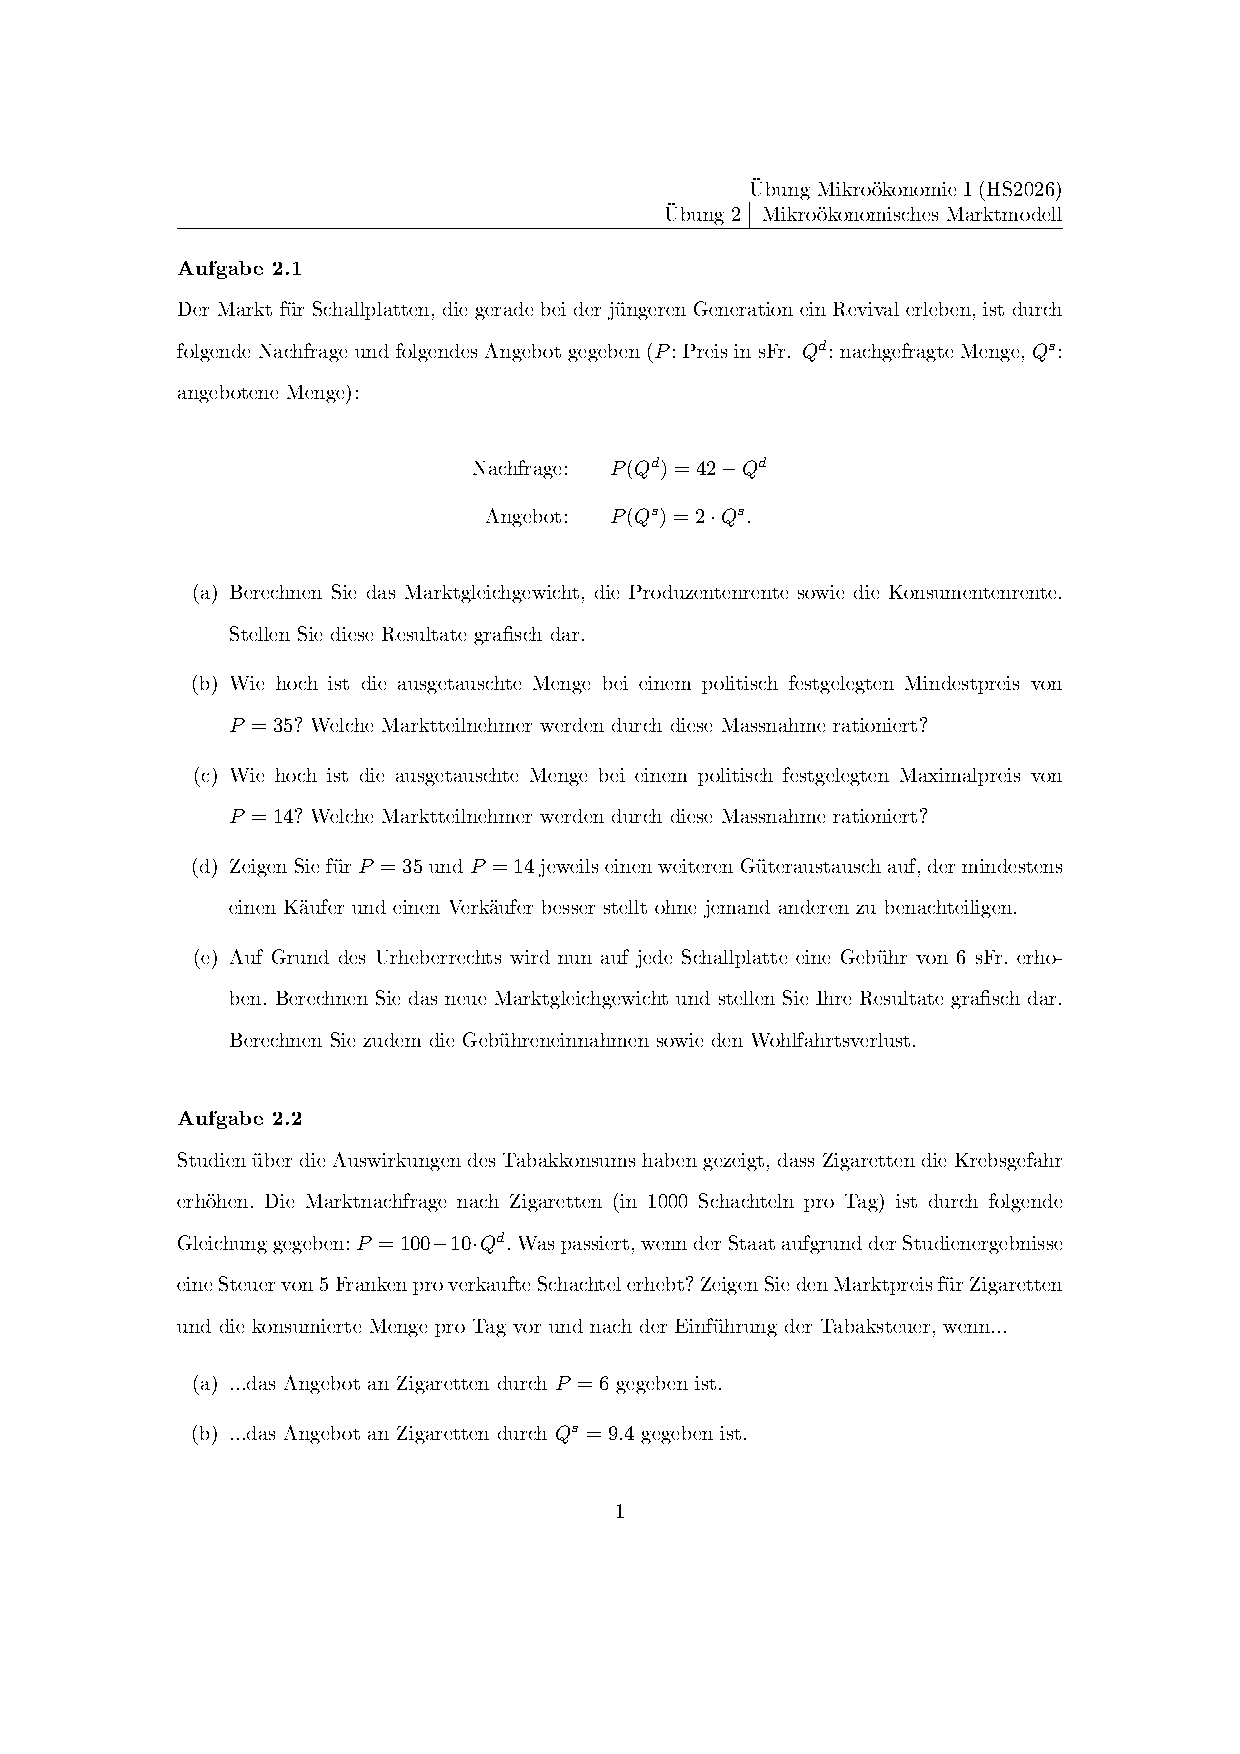
\includepdf[pages=-]{sheet.pdf}
    \exercise{2.1}
    \subexercise{a}
     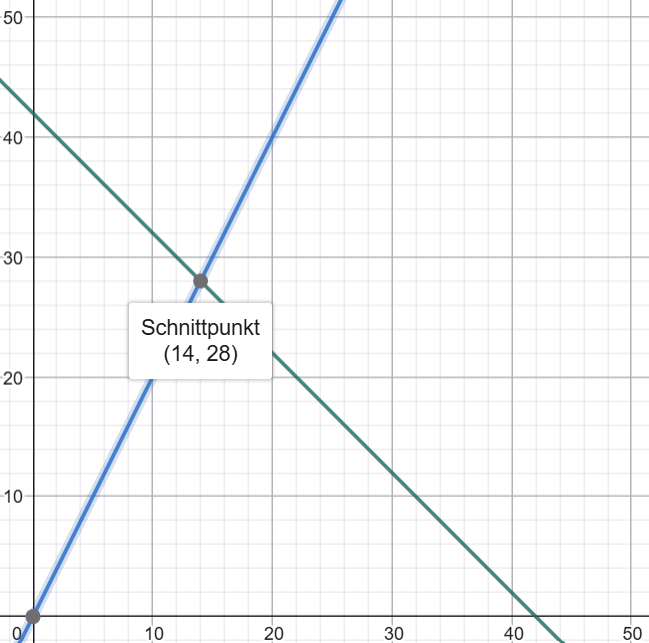
\includegraphics[width=\textwidth,height=0.7\textheight,keepaspectratio]{figures/A_Gleichgewicht.png}
    \subexercise{b}
    Es gibt Überschussangebot, Produzenten müssen rationieren. Für einen preis pro Stück von 35 sind Konsumenten im Durchschnitt bereit eine maximale menge von 7 zu konsumieren.
    Produzenten, wiederum würden für jenem Preis pro Menge, eine Menge 17.5 Produzieren
    \subexercise{c}
    Überschussnachfrage
    \subexercise{d}
    Güteraustausch von Supply bei 4 mit preis 20
    \subexercise{e}
     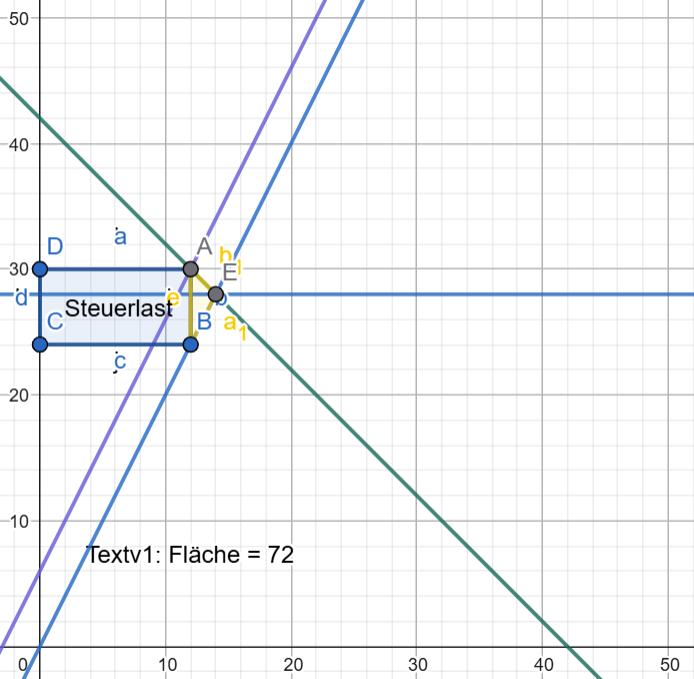
\includegraphics[width=\textwidth,height=0.7\textheight,keepaspectratio]{figures/1B_Steuer.png}
     \exercise{2.2}
     \subexercise{a}
     Angebotskurve wird um T = 5 nach oben verschoben. Keinen Einfluss für verkäufer, weil die Konsumenten die Steuerlast tragen. Es findet Wohlfahrtsverlust statt.
     \subexercise{b} 
     Angebotskurve ist senkrechte, also menge wird unabhängig vom Preis verkauft. Keinen einfluss, auf Gleichgewicht, weil Verkäufer immer zu jedem Preis verkaufen. 
    \exercise{2.3}
    \exercise{2.4}
    \subexercise{a}
    \begin{itemize}
        \item MGG: (11.33, 30.66)
        \item Steuerlast: ~90
        \item WV: 10.65
        \item PR: 128.43
        \item KR:62.23
    \end{itemize}

    \subexercise{B}
    gleich wie a

    \subexercise{C}
     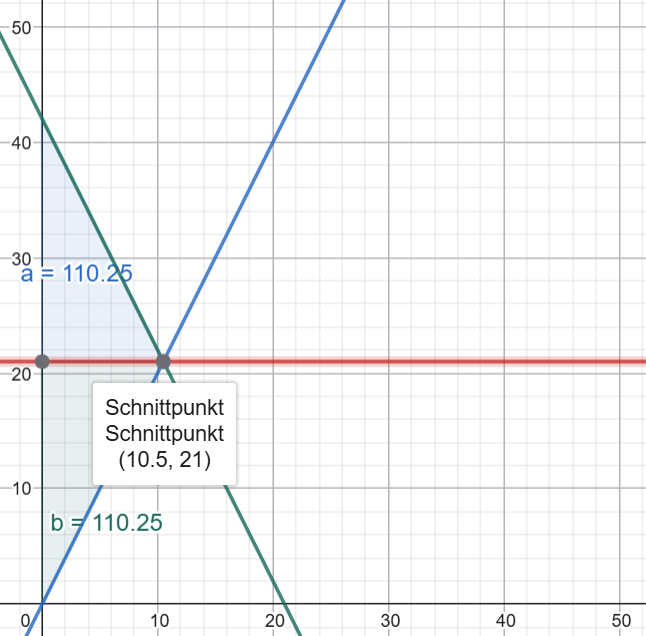
\includegraphics[width=\textwidth,height=0.7\textheight,keepaspectratio]{figures/24_c.png}

    \textbf{Steuer}
     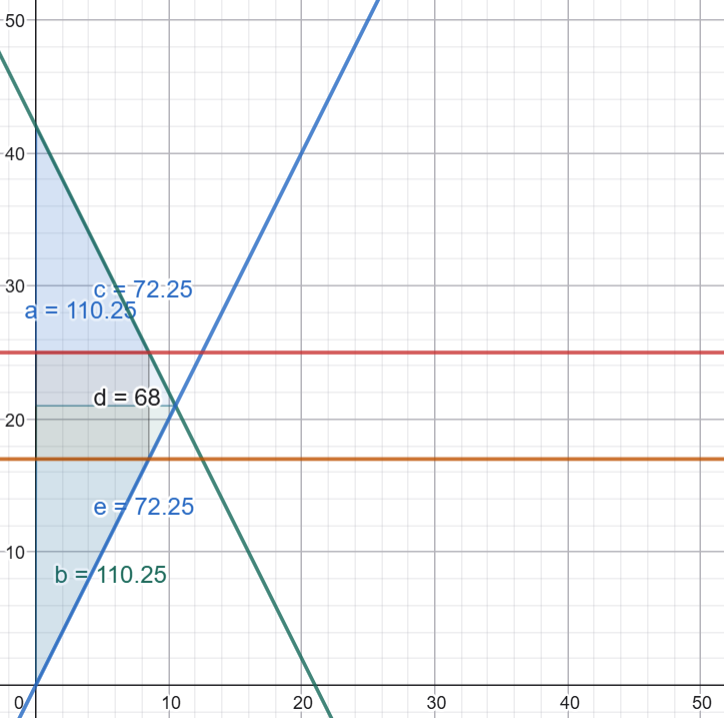
\includegraphics[width=\textwidth,height=0.7\textheight,keepaspectratio]{figures/24_c_steuer.png}
     

\end{document}
